\documentclass[../main.tex]{subfiles}

    \begin{document}
    \newpage

%%%%%%%%%%%%%%
    % Volet
    \vspace{15pt}
    %\needspace{20pt} % Réserve de l'espace
\section{Laboratoires d'innovation urbaine}

    % Block
\begin{block}[Évaluer]
    \linespread{0.9}\selectfont % Réduit l'interligne
    \emoji{bar-chart} % Emoji
    \textit{\small{Mettre en place un observatoire de l'urbanisme orienté vers les transports en commun et de l'intermodalité, destiné à évaluer les initiatives et les expérimentations.}}
\end{block}

    \begin{multicols}{2}
    \raggedcolumns
    \small{
\gras{Le développement d'organismes} dédiés à l’étude des interactions entre urbanisme et mobilité, avec une focale intermodale, vise à inscrire les quartiers de gare dans une dynamique \gras{d’expérimentation} et \gras{d’évaluation continue}. Dans une perspective de transférabilité \gras{des «~bonnes pratiques~»}, ces observatoires constitueraient des instruments d’analyse permettant d'adapter l'appui aux politiques publiques en mesurant l’évolution des pratiques et des projets urbains.
    \\\\
Au-delà de leur rôle de veille, l'opérationnalisation d'une telle \gras{structure transversale} offrirait un cadre pour \gras{tester et comparer} différentes configurations d’intégration du vélo et de la micro-mobilité dans les territoires, à travers des expérimentations en zones pilotes, tout en recueillant des données utiles. Ils contribueraient ainsi à une meilleure compréhension des facteurs influençant l’adoption des pratiques intermodales, à l'image de la conception \gras{de «~radars~» des quartiers de gare}.
    }
    %\\\\
\begin{center}
    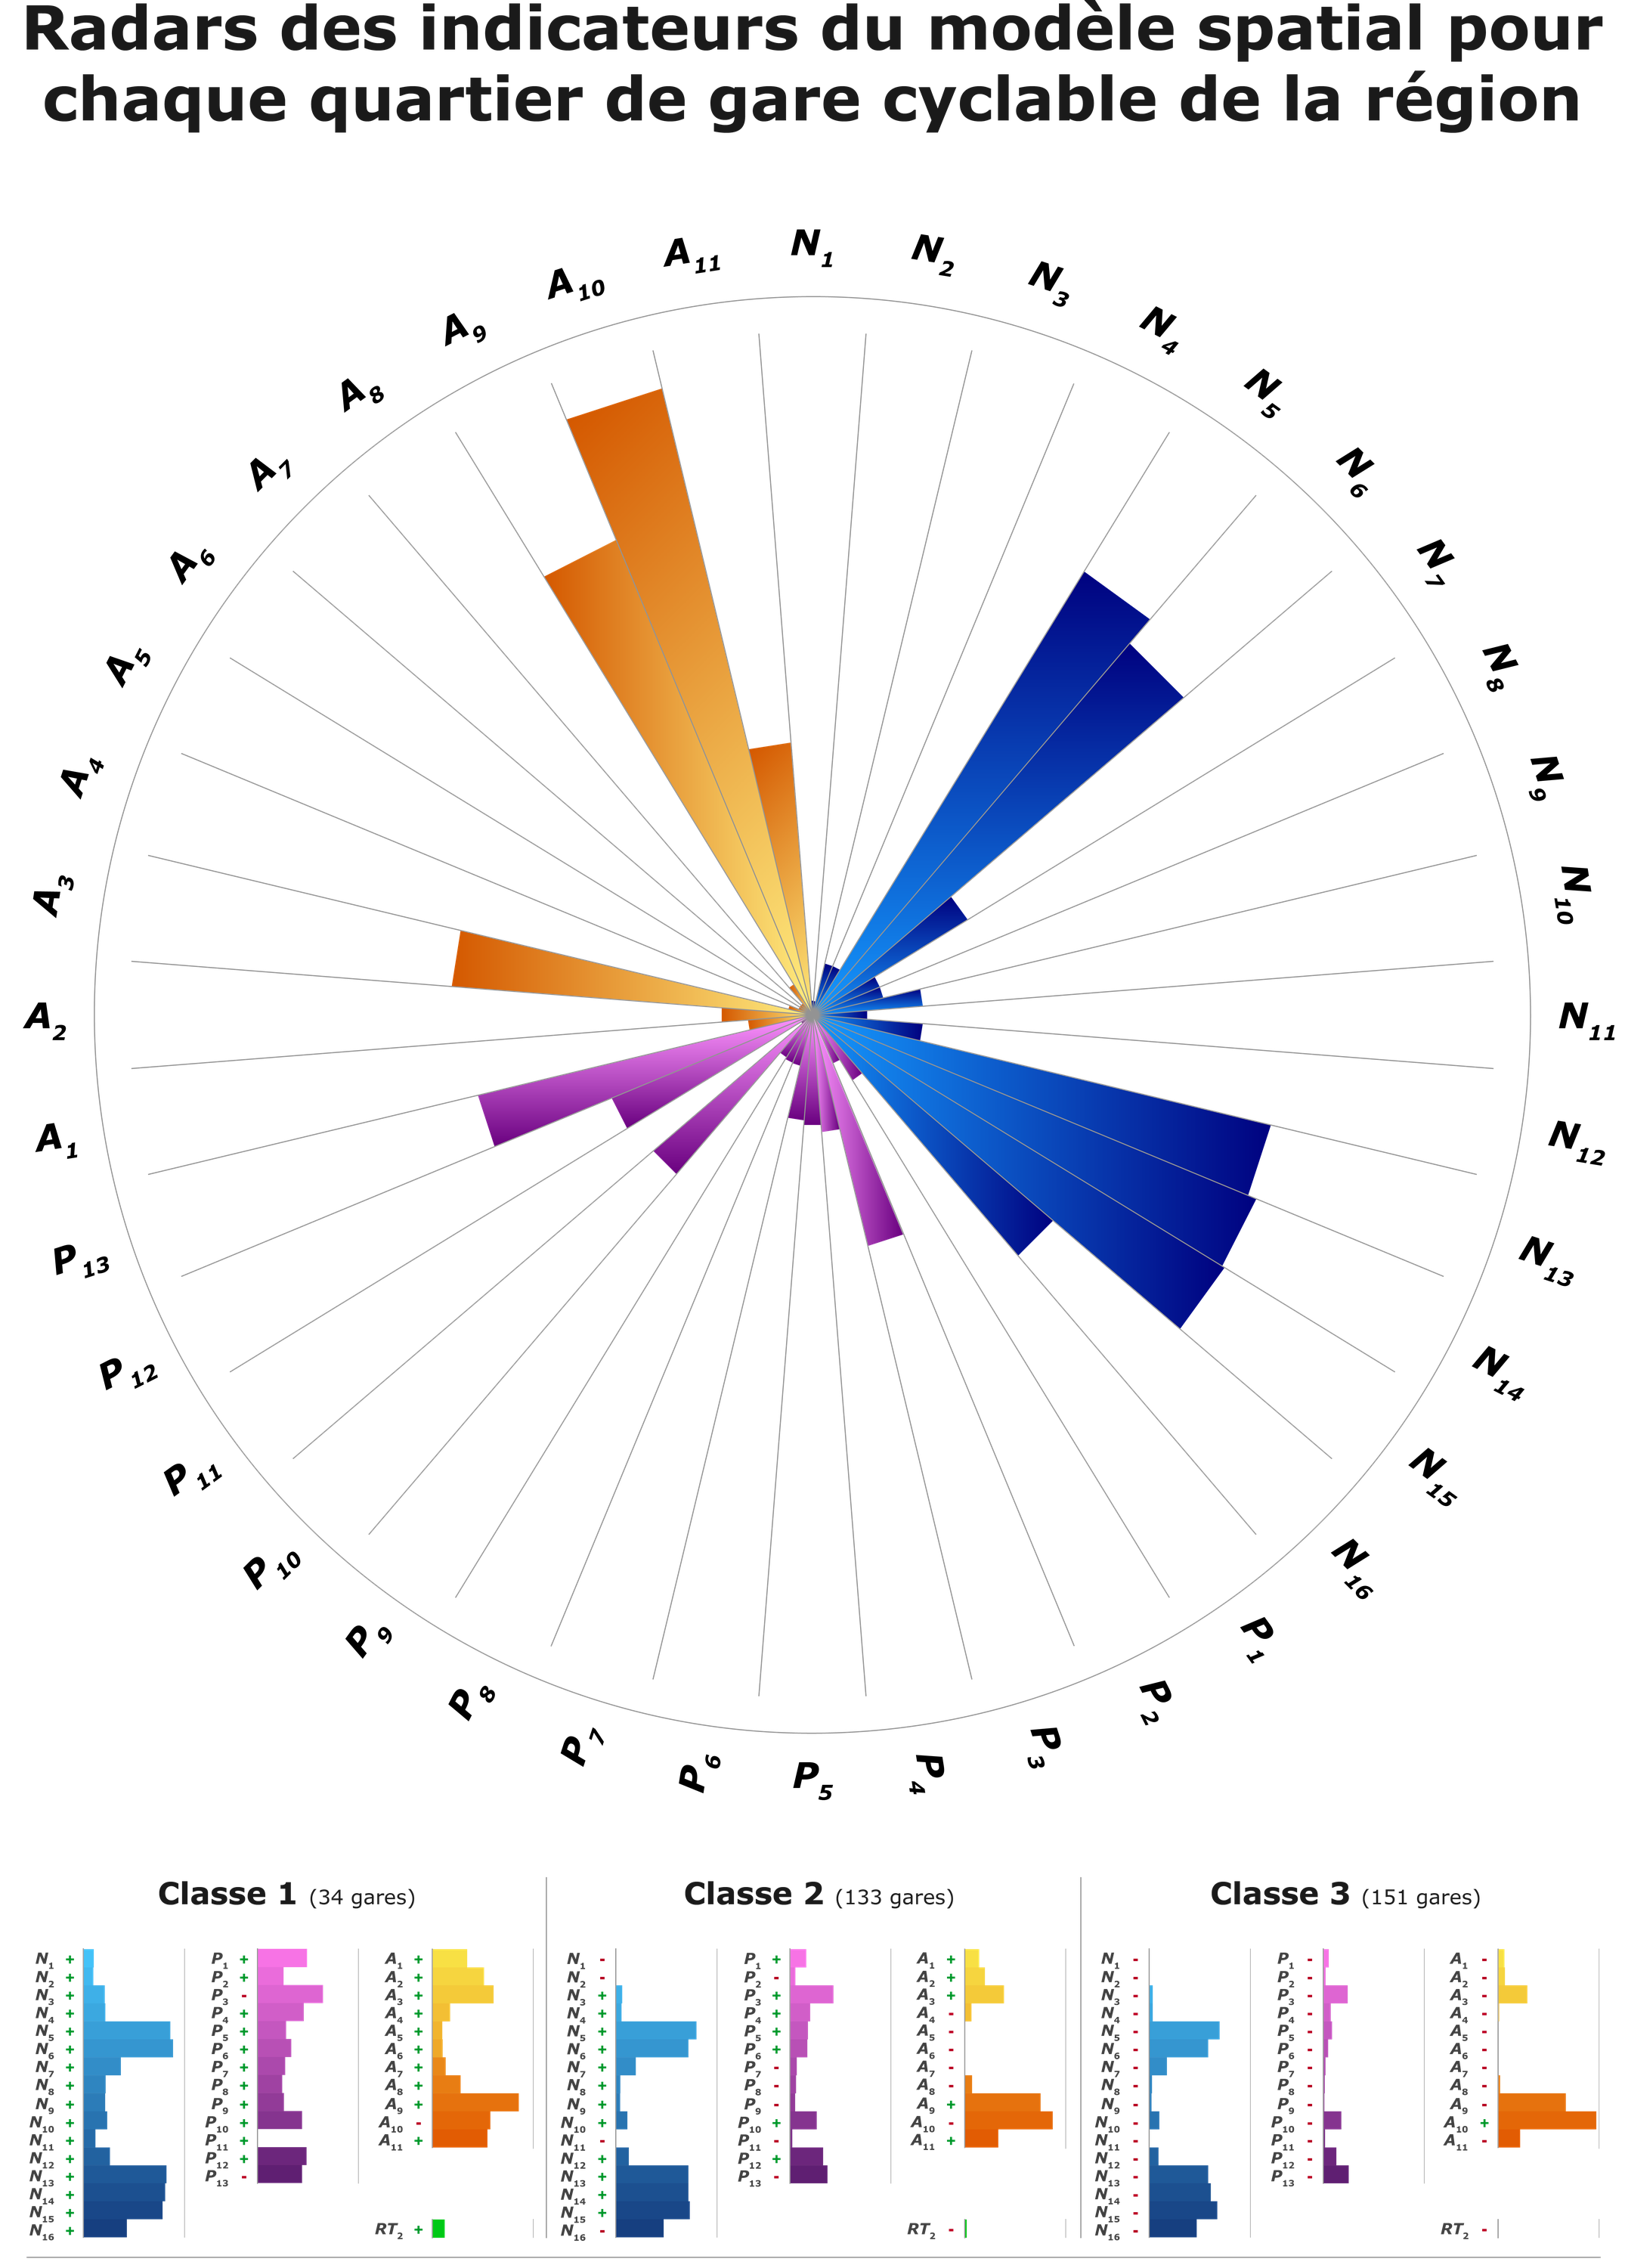
\includegraphics[width=\columnwidth]{figures/policy-brief-radar.png}
    \label{radar}
    %\vspace{-0.5cm}
    \begin{flushright}
        \begin{minipage}{1\linewidth}
            \justifying
            \noindent
            \scriptsize{\textcolor{darkgray}{Auteurs~: Dylan Moinse, Ahad Amini Pishro, Alain L'Hostis, Shiquan Zhang, Ndèye Aïta Cissé, Xavier Lehmann, Liu Yuetong, Hu Qixiao, Olivier Theureaux et Heythem Adjeroud (2025)}}
        \end{minipage}
    \end{flushright}
\end{center}

    \end{multicols}

    \end{document}